\documentclass[10pt]{article}
\usepackage{tikz}

% TikZ libraries `calc` needed now to tweak bracket.
\usetikzlibrary{backgrounds,fit}
%,decorations.pathreplacing,calc,matrix,positioning,scopes}
% Dirac Kets
\usepackage{braket}

\begin{document}
	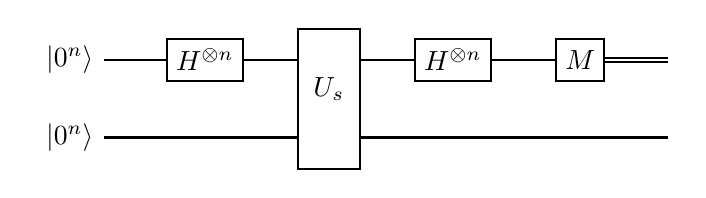
\begin{tikzpicture}[thick]
	% `operator' will only be used by Hadamard (H) gates here.
	% `phase' is used for controlled phase gates (dots).
	% `surround' is used for the background box.
	\tikzstyle{operator} = [draw,fill=white,minimum size=1.5em] 
	\tikzstyle{phase} = [draw,fill,shape=circle,minimum size=5pt,inner sep=0pt]
	\tikzstyle{surround} = [fill=blue!10,thick,draw=black,rounded corners=2mm]
	%
	\matrix[row sep=0.4cm, column sep=0.8cm] (circuit) {
	% First row.
	\node (q1) {$\ket{0^n}$}; &%[-0.5cm]
	\node[operator] (H11) {$H^{\otimes n}$}; &
	%\node[phase] (P12) {}; &
	\node[operator] (P13) {}; &
	%\node[draw,fit=(table-2-2)(table-2-3),table nodes]{F};
	\node[operator] (H11) {$H^{\otimes n}$};
	&%[-0.3cm]
	\node[operator] (M11) {$M$};
	&
	\coordinate (end1); \\
%
%
%
	% Second row.
	\node (q2) {$\ket{0^n}$}; & & \node[operator] (P23) {}; & & & \coordinate (end2);\\
	};
	\node[operator] (Us) [fit = (P13) (P23)] {$U_s$};

	% Draw bracket on right with resultant state.
%	\draw[decorate,decoration={brace},thick]
%		($(circuit.north east)-(0cm,0.3cm)$)
%		to node[midway,right] (bracket)
%{$\displaystyle\frac{\ket{000}+\ket{111}}{\sqrt{2}}$}
%		($(circuit.south east)+(0cm,0.3cm)$);
	\begin{pgfonlayer}{background}
		% Draw background box.
		%\node[surround] (background) [fit = (q1) (H31) (bracket)] {};
		% Draw lines.
		\draw[thick] (q1) -- (M11)  (q2) -- (end2);
		\draw[thick, double] (M11) -- (end1);
	\end{pgfonlayer}
	%
	\end{tikzpicture}
\end{document}

